Una barra de cobre de longitud $100\,\mathrm{cm}$ tiene difusividad térmica $1.14\,\mathrm{cm^2/s}$. Sus extremos se mantienen inicialmente a $0\,{}^\circ\mathrm C$ y se aplica calor en el centro, $x=50\,\mathrm{cm}$, manteniéndolo a $100\,{}^\circ\mathrm C$ hasta alcanzar el estado estacionario. Use el modelo unidimensional de conducción con superficie lateral aislada.

El coeficiente $1.14$ es constante. Antes de $t=0$ la fuente central divide la barra en dos tramos estacionarios sin producción interior distribuida. Después se retira la fuente y se mantiene el modelo sin pérdidas laterales. La condición inicial posterior se impone en $0<x<100$; el cambio instantáneo del extremo izquierdo no permite continuidad conjunta en $(0,0)$.

\begin{enumerate}[label=(\alph*),ref=\alph*,leftmargin=*]
\item Determine la distribución estacionaria de temperatura mientras actúa la fuente central.
\item En $t=0$ se retira la fuente central y se eleva instantáneamente el extremo izquierdo a $20\,{}^\circ\mathrm C$, manteniendo el derecho a $0\,{}^\circ\mathrm C$. Determine $u(x,t)$ para $0<x<100$ y $t>0$.
\end{enumerate}

\Needspace{8.2cm}
\begin{center}
\begin{minipage}{\linewidth}
\centering
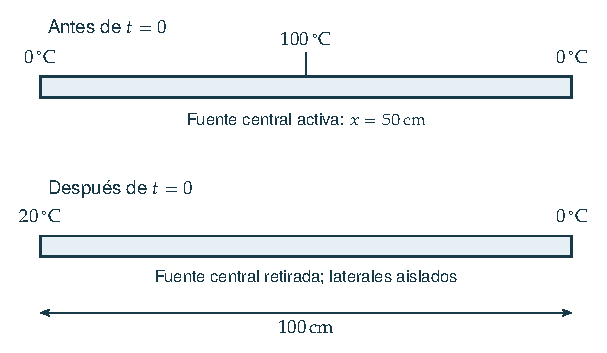
\includegraphics[width=11.52cm]{assets/M2-E0266-setup.pdf}\par
\smallskip{\small Condiciones impuestas antes y después de retirar la fuente central.\par}
\end{minipage}
\end{center}
